\documentclass[hyperref, a4paper]{article}

\usepackage{geometry}
\usepackage{float}
\usepackage{titling}
\usepackage{titlesec}
% No longer needed, since we will use enumitem package
% \usepackage{paralist}
\usepackage{enumitem}
\usepackage{footnote}
\usepackage{enumerate}
\usepackage{amsmath, amssymb, amsthm}
\usepackage{mathtools}
\usepackage{bbm}
\usepackage{cite}
\usepackage{graphicx}
\usepackage{subcaption}
\usepackage{physics}
\usepackage{tensor}
\usepackage{siunitx}
\usepackage{booktabs}
\usepackage[version=4]{mhchem}
\usepackage{tikz}
\usepackage{xcolor}
\usepackage{listings}
\usepackage{autobreak}
\usepackage[ruled, vlined, linesnumbered]{algorithm2e}
\usepackage{xr-hyper}
\usepackage[colorlinks,unicode]{hyperref} % , linkcolor=black, anchorcolor=black, citecolor=black, urlcolor=black, filecolor=black
\usepackage{prettyref}

% Page style
\geometry{left=3.18cm,right=3.18cm,top=2.54cm,bottom=2.54cm}
\titlespacing{\paragraph}{0pt}{1pt}{10pt}[20pt]
\setlength{\droptitle}{-5em}
\preauthor{\vspace{-10pt}\begin{center}}
\postauthor{\par\end{center}}

% More compact lists 
\setlist[itemize]{itemindent=17pt, leftmargin=1pt}

% Math operators
\DeclareMathOperator{\timeorder}{\mathcal{T}}
\DeclareMathOperator{\diag}{diag}
\DeclareMathOperator{\legpoly}{P}
\DeclareMathOperator{\primevalue}{P}
\DeclareMathOperator{\sgn}{sgn}
\newcommand*{\ii}{\mathrm{i}}
\newcommand*{\ee}{\mathrm{e}}
\newcommand*{\const}{\mathrm{const}}
\newcommand*{\suchthat}{\quad \text{s.t.} \quad}
\newcommand*{\argmin}{\arg\min}
\newcommand*{\argmax}{\arg\max}
\newcommand*{\normalorder}[1]{: #1 :}
\newcommand*{\pair}[1]{\langle #1 \rangle}
\newcommand*{\fd}[1]{\mathcal{D} #1}
\DeclareMathOperator{\bigO}{\mathcal{O}}
\DeclareMathOperator{\object}{Ob}
\DeclareMathOperator{\morphism}{Hom}

% TikZ setting
\usetikzlibrary{arrows,shapes,positioning}
\usetikzlibrary{arrows.meta}
\usetikzlibrary{decorations.markings}
\tikzstyle arrowstyle=[scale=1]
\tikzstyle directed=[postaction={decorate,decoration={markings,
    mark=at position .5 with {\arrow[arrowstyle]{stealth}}}}]
\tikzstyle ray=[directed, thick]
\tikzstyle dot=[anchor=base,fill,circle,inner sep=1pt]

% Algorithm setting
% Julia-style code
\SetKwIF{If}{ElseIf}{Else}{if}{}{elseif}{else}{end}
\SetKwFor{For}{for}{}{end}
\SetKwFor{While}{while}{}{end}
\SetKwProg{Function}{function}{}{end}
\SetArgSty{textnormal}

\newcommand*{\concept}[1]{{\textbf{#1}}}

\newrefformat{fig}{Figure~\ref{#1}}

% Embedded codes
\lstset{basicstyle=\ttfamily,
  showstringspaces=false,
  commentstyle=\color{gray},
  keywordstyle=\color{blue}
}

\title{Quantum Optics, Homework 3}
\author{Jinyuan Wu}

\begin{document}

\maketitle

\begin{figure}
    \centering
    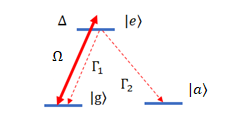
\includegraphics[width=0.4\textwidth]{fig1.png}
    \caption{A three-level $\Lambda$ system}
    \label{fig:sys-1}
\end{figure}

\paragraph{Stochastic wave function of a $\Lambda$ system} \prettyref{fig:sys-1} is a three-level $\Lambda$ system.
(a) Write down the effective Hamiltonian and quantum jump operators for \prettyref{fig:sys-1}.
(b) Suppose $\ket*{\psi_\text{s}(t=0)} = \ket*{g}$. Describe how the wave function evolves using pseudocode.
(c) Consider a case in which there is no quantum jump in $0 < t < t_0$. Find the time evolution of the 
wave function and the scattering rate 
\begin{equation}
    \gamma_1 = \expval*{C_1^\dagger C_1}{\psi_\text{s}}, \quad \gamma_2 = \expval*{C_2^\dagger C_2}{\psi_\text{s}}.
\end{equation}

\paragraph{Solution} \begin{itemize}
\item[(a)] The effective Hamiltonian is
\begin{equation}  
    H_\text{eff} = \frac{\hbar}{2} \vb*{\Omega} \cdot \vb*{\sigma} - \frac{\ii \hbar}{2} (C_1^\dagger C_1 + C_2^\dagger C_2),
\end{equation}  
where the quantum jump operators are 
\begin{equation}
    C_1 = \sqrt{\Gamma_1} \dyad*{\text{a}}{\text{e}}, \quad C_2 = \sqrt{\Gamma_2} \dyad*{\text{g}}{\text{e}}.
\end{equation}
\item[(b)] 
\end{itemize}

\paragraph{}

\end{document}